%%%%%%%%%%%%%%%%%%%%%%%%%%%%%%%%%%%%%%%%%%%%%%%%%%%%%%%%%%%%%%%
% O1-O2 events
%%%%%%%%%%%%%%%%%%%%%%%%%%%%%%%%%%%%%%%%%%%%%%%%%%%%%%%%%%%%%%%
\begin{figure*}
        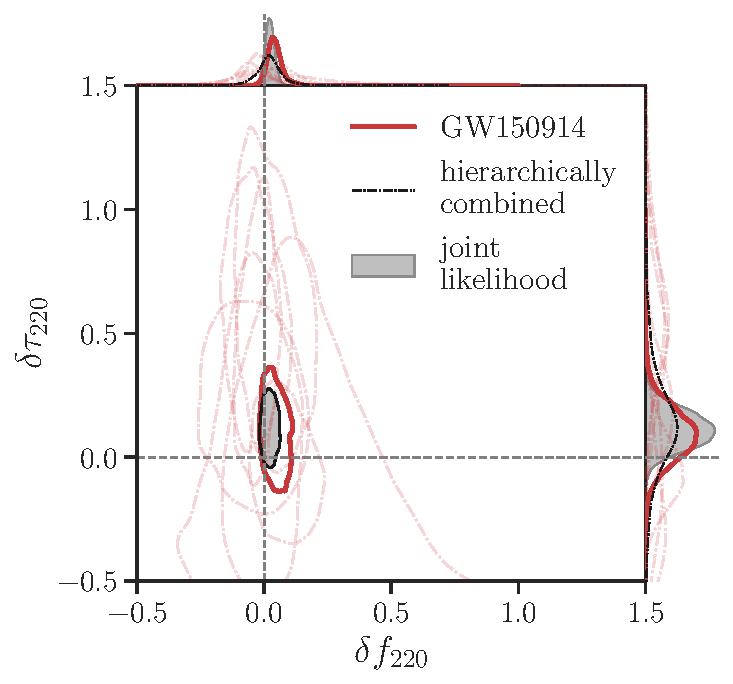
\includegraphics[width=0.5\textwidth]{figures/rin_pseob_results_v2.pdf}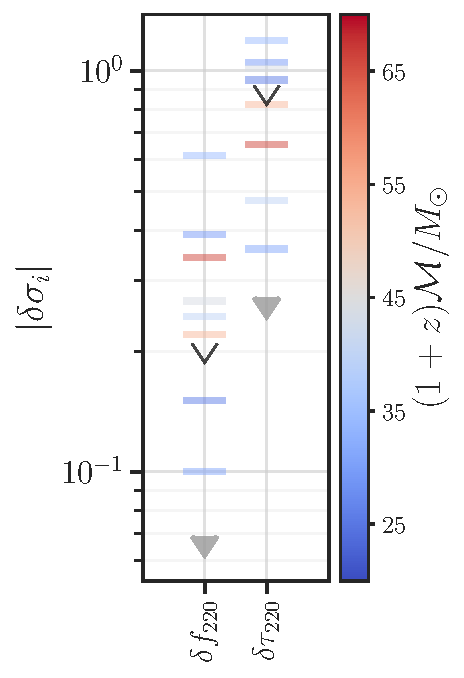
\includegraphics[width=0.3\textwidth]{figures/rin_all_events_bounds.pdf}
        \caption{\emph{Left panel}:The 90\% credible levels of the posterior probability distribution of the fractional deviations in the frequency and damping time of the $(2,\pm 2)$ QNM, $(\df{220},\dtau{220})$ and their corresponding one-dimensional marginalized posterior distributions, for events from O1, O2 and O3a passing a SNR threshold of $8$ in both the pre- and post-merger signal. The solid red curve marks the best single-event constraint, GW150914, whereas the contraints from the other events are indicated by the dash-dot curves. The joint constraints on $(\df{220},\dtau{220})$ obtained multiplying the likelihoods from individual events is given by the filled grey contours, while the hierarchical method of combination yields the black dot dashed curves. \emph{Right panel}: 90\% credible interval on the one-dimensional marginalised posteriors on $\delta \sigma_i=(\df{220},\dtau{220})$, colored by the median redshifted total mass $(1 + z)M$, inferred assuming GR. Filled gray (unfilled black) triangles mark the constraints obtained when all the events are combined by multiplying likelihoods (hierarchically).}
        \label{fig:o1o2_events}
\end{figure*}
%%%%%%%%%%%%%%%%%%%%%%%%%%%%%%%%%%%%%%%%%%%%%%%%%%%%%%%%%%%%%%%
%%%%%%%%%%%%%%%%%%%%%%%%%%%%%%%%%%%%%%%%%%%%%%%%%%%%%%%%%%%%%%%



The LIGO-Virgo Collaboration recently released their testing GR
catalogue containing results for events observed
during O3a~\cite{Abbott:2020jks}. For the test that we here present, the results shown in Ref.~\cite{Abbott:2020jks} only include events which pass a threshold for the median \sout{redshifted} \ab{detector} total mass $\geq 90 \Mo$ and SNRs in the pre- and
post-merger regions $\geq 8$~\footnote{The pre- and post-merger regions of the signal are identified from the signal's power before and after the signal reaches the peak's amplitude, which is determined from the maximum of the likelihood function obtained with the parameter-estimation analysis. The SNR values are listed in Table 4 of Ref.~\cite{Abbott:2020jks}}. 
%
The SNR threshold ensures that the signal contains sufficient information in both the inspiral and merger stages to break the degeneracy between the binary's total mass and the non-GR deviations $(\df{220}, \dtau{220})$. Such strong degeneracy is present for low-SNR events with negligible higher-modes and for which only the post-merger is detectable rendering the measurement of $(\df{220}, \dtau{220})$ impossible for those cases.\rb{should we show an example where this degeneracy happens in the appendix? We can show a corner plot with $(\df{220}, \dtau{220}, M_{\rm total })$ for 21g in the appendix for example. And perhaps also for GW150914 for comparison.}\abhi{I would be fine with this. Perhaps we should have a discussion about how best to put it in the appendix, if we decide to.} \comment{AB: I would agree in showing the two plots that are at the end of the paper in a short Appendix B.}
On the other hand the total mass threshold $\geq 90 \Mo$ was employed due to the fact that this analysis is computationally expensive, and also because we expected these events to be the most promising for ringdown studies. However, since the SNR threshold alone should be sufficient for the analysis, for this paper we run the test on all the events listed in Ref.~\cite{Abbott:2020jks} that have SNRs in the pre- and post-merger regions $\geq 8$, without imposing any mass threshold.

\ab{Given the above we add the signals}  GW190630$\_$185205 and GW190828$\_$063405, to the list of GW events considered in Ref.~\cite{Abbott:2020jks}. \ab{Furthermore, for the first time, 
we apply our method to measure the QNMs to GW events from O1 and O2, notably GW150914 and GW170104.} The other high-mass events from O1 and O2, GW170729, GW170809,
GW170814, GW170818 and GW170823 do not have an SNR $\geq 8$ in the
merger-ringdown signal. The list of the signals for which we run the analysis is given in Table~\ref{tab:qnm_o1o2_results}~\footnote{See Table IV of Ref.~\cite{Abbott:2020jks} for a list of the SNR
  thresholds. The paper quotes them for the purpose of the IMR
  consistency test, but the same thresholds have been used for the
  $\pSEOB$ test, as well.}.
  
For all the relevant signals, we show the posterior distributions
$(\df{220}, \dtau{220})$ in the left panel of
Fig.~\ref{fig:o1o2_events} and also provide the reconstructed QNM
parameters, $(\fngr{220}, \taungr{220})$ in
Table~\ref{tab:qnm_o1o2_results}. \comment{AB: could you explain how the mass 
and spin in Table II are computed? I think we should also list the mass and 
spin fron NR fits.} In the right panel of
Fig.~\ref{fig:o1o2_events} we also provide a summary of the 90\%
credible intervals on the 1D marginalized posteriors. We highlight the
dependence of the constraints on the total mass of the
system. In general, the tightest bounds are set by the 
most massive systems, as they tend to have larger post-merger SNR. We
find a similar trend in the right panel of Fig.~\ref{fig:o1o2_events}.
 
Among all the GW signals detected so far, GW150914 (solid curve in
Fig.~\ref{fig:o1o2_events}) is unique in its loudness, leading to the
first, and to date, best attempt in measuring the QNM
frequencies~\cite{TheLIGOScientific:2016src,Brito:2018rfr,Carullo:2019flw,Isi:2019aib}. Within
90\% credibility we obtain from GW150914:
%
\begin{equation}\label{GW150914_delta}
\df{220}=0.04^{+0.06}_{-0.04}\,\quad \dtau{220}=0.09^{+0.18}_{-0.18}\,.
\end{equation}

Stronger constraints can be obtained by combining information from all the events~\cite{Abbott:2020jks}. If we assume that the fractional deviations $(\df{220},\dtau{220})$ take the same values in multiple events, we can assume
the posterior of one event to be the prior for the next, and obtain a
joint posterior probability distribution. For $N$ observations, where
$P_j(\df{220}, \dtau{220} | d_j)$ is the posterior for the $j$-th
observation corresponding to the data set $d_j$, $j=1,\dots,N$, the joint
posterior is given by:
%
\begin{equation}
P(\df{220}, \dtau{220} | \{d_j\}) = P(\df{220}, \dtau{220}) \prod _{j=1}^N \frac{P(\df{220}, \dtau{220} | d_j) }{P(\df{220}, \dtau{220})}
\end{equation}
%
where $P(\df{220}, \dtau{220})$ is the prior on $(\df{220},
\dtau{220})$. However, since here we assume the prior on $(\df{220},
\dtau{220})$ to be flat (or uniform), the joint posterior is equal to
the joint likelihood. We show these joint likelihoods on $(\df{220}, \dtau{220})$, as well as, the corresponding 1D marginalized distributions as filled grey curves in Fig.~\ref{fig:o1o2_events}. From the joint likelihood we obtain within 90\% credibility: 
%
\begin{equation}
\df{220}=0.02^{+0.03}_{-0.03}\,,\quad \dtau{220}=0.11^{+0.12}_{-0.12}\,.
\end{equation}
%

\ab{However, the deviations parameters $(\df{220},\dtau{220})$ depend in general on the source's parameters, so they are not constant across the GW signals observed by LIGO and Virgo.}
As described in Ref.~\cite{Abbott:2020jks}, we can relax the assumption of a \sout{shared} \ab{constant} deviation across all events by using the hierarchical inference technique originally proposed in Refs.~\cite{Zimmerman:2019wzo,Isi:2019asy}. The general idea behind this technique is to assume that the non-GR parameters $(\df{220},\dtau{220})$ are drawn from a common underlying distribution, whose properties can be inferred from the population of events. Following~\cite{Zimmerman:2019wzo,Isi:2019asy,Abbott:2020jks} we model the population distribution with a Gaussian  $\mathcal{N}(\mu,\sigma)$ of unknown mean $\mu$ and standard deviation $\sigma$. Under those assumptions, the goal is then to directly measure a posterior distribution $P(\mu, \sigma |  \{d_j\}) $ for $\mu$ and $\sigma$ from a joint analysis of all the GW events. If GR is correct, then this posterior should be consistent with $\mu=0$ and $\sigma=0$. From Bayes' theorem it follows that~\cite{Isi:2019asy}:
%
\begin{equation}
P(\mu, \sigma |  \{d_j\}) \propto P(\mu,\sigma)\prod _{j=1}^N P(d_j |\, \mu, \sigma) \,,
\end{equation}
%
where $P(\mu,\sigma)$ is the prior (also known as hyperprior) on ($\mu,\sigma$), and $P(d_j | \mu, \sigma) $ can be written in terms of the individual likelihoods of a given non-GR parameter $\xi_{\text{nGR}}$ using~\cite{Isi:2019asy}
%
\begin{equation}
P(d_j | \mu, \sigma) = \int P(d_j |\, \xi_{\text{nGR}})  P(\xi_{\text{nGR}} |\, \mu, \sigma) \,d\xi_{\text{nGR}} \,.
\end{equation}
%
Here $P(\xi_{\text{nGR}} | \,\mu, \sigma) = \mathcal{N}(\mu,\sigma)$ by construction and $P(d_j |\, \xi_{\text{nGR}})$ is the likelihood for the parameter $\xi_{\text{nGR}}$ for a given event $d_j$ that is computed from the standard parameter estimation analysis. After obtaining $P(\mu, \sigma |  \{d_j\})$, we can then infer a population distribution for a given non-GR parameter $\xi_{\text{nGR}}$ using~\cite{Isi:2019asy}:
%
\begin{equation}\label{hier_combine}
P(\xi_{\text{nGR}} | \{d_j\}) = \int P(\xi_{\text{nGR}} |\, \mu, \sigma)\,P(\mu, \sigma |  \{d_j\})\,d\mu\,d\sigma \,.
\end{equation}
%
Notice that, if we fix $\sigma=0$, this approach is equivalent to assume that all events share the same non-GR parameter $\xi_{\text{nGR}} =\mu$ and Eq.~\eqref{hier_combine} reduces to the joint likelihood~\cite{Zimmerman:2019wzo}. In practice, we use the \texttt{stan}-based code~\cite{stan} developed and used in Refs.~\cite{Isi:2019asy,Abbott:2020jks} to obtain $P(\mu, \sigma |  \{d_j\}) $ and compute $P(\xi_{\text{nGR}} | \{d_j\})$.

The 1D posteriors for $\df{220}$ and $ \dtau{220}$ obtained with this technique are shown in Fig.~\ref{fig:o1o2_events} (dash-dotted curves) with corresponding median and 90\% credible interval given by: 
%
\begin{equation}
\df{220}=0.02^{+0.09}_{-0.09}\,,\quad \dtau{220}=0.13^{+0.42}_{-0.40}\,.
\end{equation}
Compared to Ref.~\cite{Abbott:2020jks} these constraints are almost a factor $\sim 4$ more stringent for $\df{220}$ and a factor $\sim 2$ for $\dtau{220}$. Similar improvements hold for the hyperparameters: $\df{220}\,(\mu=0.02^{+0.05}_{-0.05},\,\sigma<0.09)$ and $\dtau{220}\,(\mu=0.13^{+0.20}_{-0.18},\,\sigma<0.38)$.


%%%%%%%%%%%%%%%%%%%%%%%%%%%%%%%%%%%%%%%%%%%%%%%%%%%%%%%%%%%%%%%
% Table for LVC values
%%%%%%%%%%%%%%%%%%%%%%%%%%%%%%%%%%%%%%%%%%%%%%%%%%%%%%%%%%%%%%%
\begin{table}

\begin{tabular}{lllll}
\toprule
Event & $\fngr{220}$ (Hz) & $\taungr{220}$ (ms) & $M_f/\Mo$ & $a_f$ \\[0.075cm]
\midrule
\hline

GW150914 &
$258^{+17}_{-13}$ &
$4.5^{+1.1}_{-0.9}$ &
$71^{+9}_{-10}$ &
$0.8^{+0.1}_{-0.2}$
\\[0.075cm]

GW170104 &
$291^{+15}_{-30}$ &
$5.5^{+3.5}_{-2.4}$ &
$74^{+11}_{-20}$ &
$0.9^{+0.1}_{-0.4}$
\\[0.075cm]

GW170729 &
$152^{+13}_{-9}$ &
$10.7^{+4.2}_{-3.7}$ &
$141^{+20}_{-29}$ &
$0.9^{+0.1}_{-0.2}$
\\[0.075cm]

GW190519\_153544 &
$124^{+12}_{-13}$ &
$10.3^{+3.6}_{-3.1}$ &
$155^{+24}_{-30}$ &
$0.8^{+0.1}_{-0.3}$
\\[0.075cm]

GW190521\_074359 &
$205^{+15}_{-12}$ &
$5.3^{+1.5}_{-1.2}$ &
$86^{+12}_{-14}$ &
$0.7^{+0.1}_{-0.3}$
\\[0.075cm]

GW190630\_185205 &
$248^{+32}_{-53}$ &
$3.9^{+2.4}_{-1.8}$ &
$66^{+19}_{-42}$ &
$0.6^{+0.3}_{-0.6}$
\\[0.075cm]

GW190828\_063405 &
$258^{+201}_{-28}$ &
$4.2^{+4.2}_{-1.9}$ &
$67^{+26}_{-30}$ &
$0.8^{+0.2}_{-0.7}$
\\[0.075cm]

GW190910\_112807 &
$174^{+12}_{-8}$ &
$9.5^{+3.1}_{-2.7}$ &
$123^{+15}_{-18}$ &
$0.9^{+0.0}_{-0.1}$
\\[0.075cm]

\bottomrule
\end{tabular}
\caption{The median and symmetric 90\% credible intervals of the frequency and damping time of the $(2,\pm2)$ QNM, and the mass and spin of the remnant object estimated from 
the QNM frequencies \ab{using the $\pSEOB$ model.} \comment{AB: I would add the mass and spin of the remnant from NR fits, as well. The final mass should be multiplied by $(1+z)$. Correct?}}
\label{tab:qnm_o1o2_results}
\end{table}

%%%%%%%%%%%%%%%%%%%%%%%%%%%%%%%%%%%%%%%%%%%%%%%%%%%%%%%%%%%%%%%
%%%%%%%%%%%%%%%%%%%%%%%%%%%%%%%%%%%%%%%%%%%%%%%%%%%%%%%%%%%%%%%
